\chapter{Conclusions}


Starting from the theoretical foundation of the interest rate subject, the thesis grows step by step in order to let the reader understanding the bootstrapping procedure and its limits which are outmoded by the introduction of the abcd framework. Moreover, it provides innovative empirically based contents enlarging the current literature.\\
The advantages of the tenor based approach with respect to the legacy framework and the further developments of the thesis are exposed.
If compared with the bootstrapping procedure, which is currently employed by the practitioners, the abcd model, although relying on it, is:

\begin{itemize}
    \item parsimonious: it allows to  describe with few parameters what currently it needs a bootstrapping procedure, where each point of the grid curve is a parameter, to be retrieved;
    \item interpolation independent: thanks to the functional form does not need an interpolation algorithm to retrieve the not quoted grid points which is a huge advantage thinking at the smoothness problem which comes with numeric procedure and the possible computational misleading results;
    \item smoothness: a key point of the model is the $C^{2}$ property of the abcd functional form, which by construction solves the shape problems. Besides, if employed together with not incremental calibration it perfectly matches with the natural smoothness which belongs to the ON curve;
    \item information short: at the beginning of the curve, if the $x$ tenor is greater than ON, implying that the first available instrument insists on the $x$ date, not perfect manipulation can accumulate errors which explode in such part of the curve invalidating it. Once again, the functional form of the basis overcomes them;
    \item meaningful parameters: with respect to the bootstrapping procedure, the parameters are easy to be interpreted making easier to understand both the indication and the matter related to the model;
\end{itemize} 

If compared with an ideal text book framework, the only one drawback is the impossibility to exact reprice the market quotes, it is not possible to reprice with 4 parameters a market which needs at least n greater than 4 parameters to be exactly repriced. Anyway, it is a sort of ``uroboros": in order to perfectly reprice the market it is needed a really flexible structure such as a bootstrapped curve, on the other hand it cannot have the ideally smoothness which a functional basis can provide. There is an explanation, the market is not perfectly smooth, the quotes are not updated, for instance the futures, with a continuous step and temporal skews exist on the market, for these reasons an abcd model is an extremely good proxy of the market once eliminated the noise which comes with it. The described behaviour it can be recognized thinking at the k correction factors, which allows to perfectly reprice the market quotes negotiating exact fitting for smoothness.
An example is available observing the 6M simple forward curve and comparing the legacy

\begin{figure}[H]
\centering
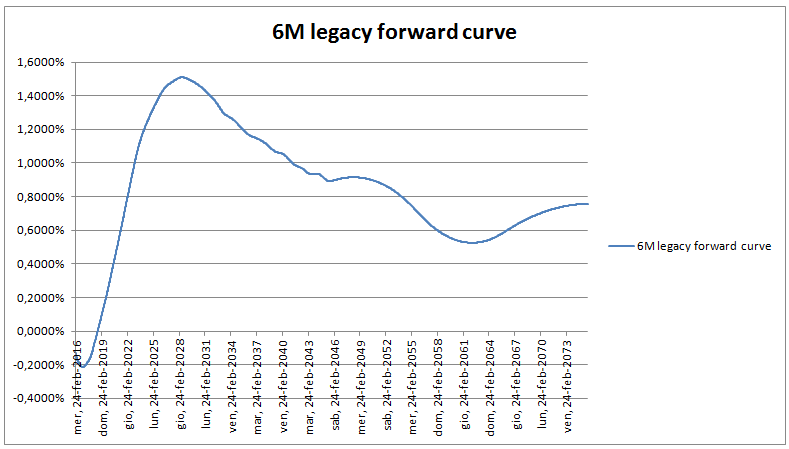
\includegraphics[scale=0.6]{6Mlegacyfroward}
\caption{6M simple forward from 6M legacy curve}
\label{fig:6Mlegacyfroward}
\end{figure}

with the acdt

\begin{figure}[H]
\centering
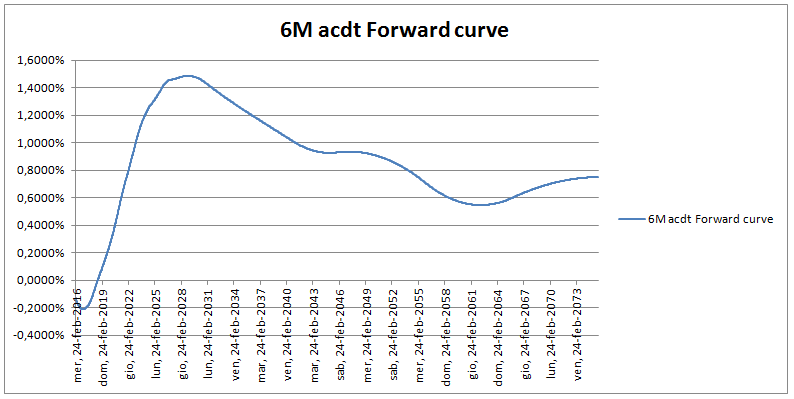
\includegraphics[scale=0.6]{6Macdtfroward}
\caption{6M simple forward from 6M acdt}
\label{fig:6Macdtfroward}
\end{figure}

and the corrected acdt

\begin{figure}[H]
\centering
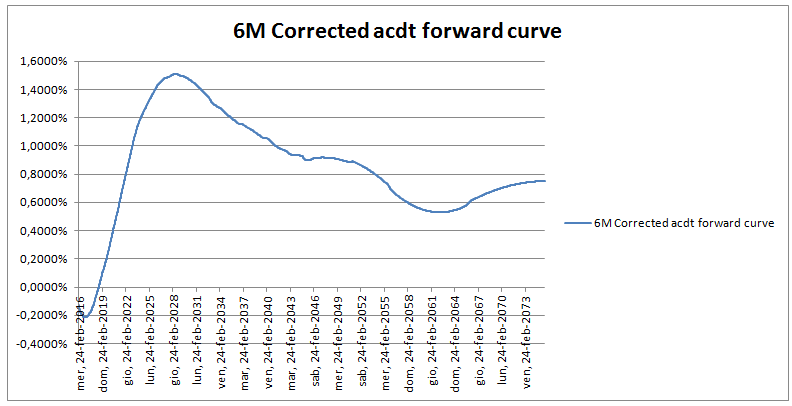
\includegraphics[scale=0.6]{6Mcorrectedacdtfroward}
\caption{6M simple forward from 6M corrected acdt}
\label{fig:6Mcorrectedacdtfroward}
\end{figure}

which looks exactly the same once excluded the noise.
The choice between them should be commensurate to the purpose, a broker would use the acdt without correction in order to perfectly reprice few market quotes and assuming an acdt shape for the not liquid ones. A market maker would use or the bootstrapped curve either the corrected acdt for exactly repricing the observed quotes.
In the specific case they both use acdt instead of abcd model because of the basis shifting property together with the financial common time of maximum assumption.

In order to assess the innovative contents with respect to the abcd framework the acdt features are enlisted:

\begin{itemize}
    \item preservation of the abcd features;
    \item shared basis time of maximum across different tenors and type of basis: the uncertainty is not a tenor function, but  it is exogenously event driven, therefore it is possible to contingently describe the basis time of maximum of different tenor based curve;
    \item additive basis: common exponential decay factor allows to shift from absolute to relative basis reconciling the incremental and not incremental calibration. It resolves the impasse which was created such that either the relative or the absolute basis can be abcd, that it was not making sense, because empirically both of them were well fitted with an abcd curve and it was only a mathematical reconciliation problem. The possibility to move from/to absolute basis to/from relative basis brings a tangible computational advantage, just one curve is bootstrapped, while 4 basis calibrated and 4 trivial set of operations are needed to retrieve the remaining 3 basis;
    \item new input form: improved capability of the model to elaborate information. It is possible to derive the thesis conclusion also without using an acdt thanks to the linearity property among $a$ and $b$. Anyway is far easier to interpret the outputs in term of basis maximum and time of maximum relation more than in term of $b$ and $c$ parameters.
\end{itemize} 

Together with the progress come also two points which are less stable and more difficult to justify than the previous ones:

\begin{itemize}
    \item common value for the decay parameter $c$: it is difficult to evaluate whether or not the $c$ value should be the same for each tenor based curve, a logical deduction can make it more acceptable. If it is sane to force a same maximum point of uncertainty and if it is safe to suppose a common long run value $d$, the part of curve for a generic tenor $x$ which lays between these moments should have a similar dynamics $c$ influenced by a proper one explained by $a_{x}$ and $b_{x}$. Following the same ratio, it makes sense that for reaching the peak of uncertainty in the same point of time a certain relation should exist between different curve and it is the one among the i-th $a$ and $b$.
    \item abcd-ness of the relative basis: considering that with the new framework all the relative basis can be retrieved with respect to an $x$ tenor (in the specific case 6M) it makes sense that the previous rationale is still valid. Besides, a rationale can also be found by construction: given that the relative basis inherits the decaying behaviour from the relative ones, and without considering the basis on the 1M which is a mutation of the ON one, the $d$ value goes to zero by construction therefore it makes sense that the basis time of maximum is in the same point of time of the absolute basis one and by construction an implied constraint of their a and $b$ is needed.
    \item$s_{x,y}(t_{max})$ as difference of $s_{x}(t_{max})$ and $s_{y}(t_{max})$: implication which is empirically valid because of the model hypothesis and maybe too  compelling.
\end{itemize} 

Before leaving the reader the Author wants to indicate the remaining points which should be explored on the topic:

\begin{itemize}
    \item to test the model with the current dataset;
    \item calibration on basis swaps and computation of the sensitivities w.r.t. them because they are the instruments which better reflect the basis movements;
    \item k adjustment just for staying in the bid ask, not exact repricing;
    \item to test the model at least on another currency (dollar);
    \item model generalization adding more parameters;
\end{itemize}

Concluding, despite the presence of points of debate which are still open, the Author thinks the model works and absolves its noble function: it gathers information from external sources and after reworking them relying on both real world intuitions and model expedients it gives back signals and insights to the user which understands its merits and defects, remembering that a model is just a comfortable but not an exact world representation.

